\documentclass{report}
\usepackage{graphicx}
\usepackage[portuguese]{babel}
\usepackage[utf8]{inputenc}
\usepackage{hyperref}
\usepackage{indentfirst}
%\usepackage[latin1]{inputenc}
%\usepackage{url}
\usepackage{color}
\usepackage{enumerate}
\usepackage{alltt}
\usepackage{fancyvrb}
\usepackage{listings}
\usepackage{amsmath}
\newcommand{\keyword}[1]{\textsf{#1}}

\DefineVerbatimEnvironment{code}{Verbatim}{fontsize=\footnotesize}
%LISTING - GENERAL
\lstset{
	basicstyle=\small,
	numbers=left,
	numberstyle=\tiny,
	numbersep=5pt,
	breaklines=true,
    frame=tB,
	mathescape=true,
	escapeinside={(*@}{@*)}
	}


\title{Processamento de Linguagens e Compiladores\\ (3º ano de LCC)\\ \textbf{Desenvolvimento de Linguagem de Programação Imperativa}\\ TP3\\ Grupo 09}
\author{Filipe Barbosa\\ A77252 \and  Hugo Ferreira\\ A78555 \and Nuno Morais\\ A77368 }
\date{\today}

\begin{document}
	
\maketitle
	

\begin{abstract}
	Neste relatório apresentamos a linguagem que criamos chamada gram e o compilador que gera o código para a Máquina Virtual VM.
\end{abstract}

\tableofcontents

\chapter{Introdução} \label{intro}
\section{Intrudução}
\indent
Neste relatório apresentamos o ultimo trabalho pratica da UC de PLC. O trabalho consistia em desenvolver um processador de linguagens e desenvolver, tambem, um compilador que gera o codigo para uma maquina virtual. Para a realização deste trabalho usamos a ferramenta Yacc para gerar compiladores baseados em gramaticas tradutoras.

\chapter{Gramatica e Compilador} \label{fi}
\section{Descrição informal do problema}
\indent
Neste trabalho foi pedido para criarmos uma linguagem de programação imperativa e desenvolver um compilador para a linguagem criada.\\
\indent
Na linguagem as declarações de variáveis devem ser colocadas no início do programa, não pode haver re-declarações e não se pode usar variáveis sem estar declaradas primeiro. Caso não seja atribuido um valor à variável depois da declaração, esta ficará com o valor zero se for um inteiro, se for um float ficará 0.0 e se for string ficará $"$".\\
\indent  	
O compilador deve gerar o código assembly para a Máquina Virtual VM.

\section{Especificação dos requisitos}
\indent
Para este trabalho a linguagem que criamos tem de conter os seguintes requisitos:
\begin{enumerate}
	\item Declarar variaveis atomicas dos tipos Inteiro, Real e Boleano.
	\item Ler do standard input e escrever no standard output.
	\item Conter condiçoes e ciclos repetir...até.
    \item Gerar codigo Assembly para a VM.
\end{enumerate}

\section{Expressões regulares} 
As expressões regulares usadas foram:

\begin{enumerate}
	\item $[$=$\backslash$+$\backslash$-$\backslash$*$\backslash$/\%()$<>$!,;]
	\item $[$a-zA-Z][a-zA-Z0-9]*
	\item $\backslash$"[\^\"]* $\backslash$"
	\item -?$[$0-9]+
	\item -?$[$0-9]+$\backslash$.[0-9]+ 
	\item while$|$WHILE
	\item if$|$IF 
	\item else$|$ELSE
	\item $[$ $]$+AND$[$ $]$+
	\item $[$ $]$+OR$[$ $]$+
	\item $\backslash$$<=$
	\item $\backslash$$>=$
	\item ==
	\item != 
	\item $[$$\backslash$t$\backslash$n]

\end{enumerate}

\section{Linguagem}
\subsection{Gram}
\indent
Como referido anteriormente, foi-nos pedido que criassemos uma linguagem de programação. Para o desenvolvimento da linguagem inspiramo-nos na pseudo linguagem usada nas aulas.\\
\indent
Para definir a nossa linguagem usamos uma gramatica independente de contexto.\\
\indent
A linguagem Gram reconhece os tipos: numeros inteiros(int), numeros decimais(float) e sequencia de caracteres(string).
Para comparação usa-se os simbolos usuais: $<=$, $>=$, $<$, $>$, $==$ e $!=$. Utiliza-se "AND" e "OR" como simbolos de operadores logicos.

\indent
A nossa linguaguem está definida pela eguinte GIC:

\begin{code}

    1 Prog: Prog If
    2     | Prog While
    3     | Prog Atrib ';'
    4     | Prog VAR '=' Expr ';'
    5     | Prog Func ';'
    6     | %empty

    7 Func: VAR Expr

    8 Atrib: TYPE VAR
    9      | Equal

   10 Equal: TYPE VAR '='
   11      | Equal Expr

   12 If: IF Cond
   13   | IF '{' Prog '}' ELSE
   14   | IF '{' Prog '}'

   15 While: WHILE
   16      | WHILE Cond
   17      | WHILE '{' Prog '}'

   18 Cond: NUMI
   19     | '(' Expr EQUALS Expr ')'
   20     | '(' Expr NE Expr ')'
   21     | '(' Expr '<' Expr ')'
   22     | '(' Expr '>' Expr ')'
   23     | '(' Expr LE Expr ')'
   24     | '(' Expr GE Expr ')'
   25     | '(' Cond AND Cond ')'
   26     | '(' Cond OR Cond ')'
   27     | '!' Cond

   28 Expr: '(' Expr '+' Expr ')'
   29     | '(' Expr '-' Expr ')'
   30     | '(' Expr '*' Expr ')'
   31     | '(' Expr '/' Expr ')'
   32     | '(' Expr '%' Expr ')'
   33     | '(' Expr ')'
   34     | Exp

   35 Exp: NUMI
   36    | NUMF
   37    | STR
   38    | Func

\end{code}

\chapter{Codificação}
\section{Problemas de implementação}
\indent
Como esperado, deparamo-nos com vários problemas na implentação do codigo durante a realização deste trabalho prático, sendo que alguns deles acabaram por não ser solucionados.

\chapter{Conclusão} \label{concl}
 \indent
 Para a realização deste trabalho foi necessario o uso da maior parte da materia lecionada ao longo deste semestre. Através do conhecimento adquirido nas aulas sbore GIC's e sobre o gerador Yacc e Flex criamos um compilador para converter a nossa linguagem em pseudo-codigo para a maquina virtual VM. Não conseguimos realizar todas as tarefas propostas pelo professor.
 \indent
 Como trabalho futuro gostariamos de conseguir acabar as tarefas que não conseguimos acabar.

\appendix
\chapter{Imagens}

\begin{figure}[ht]
	\centering
	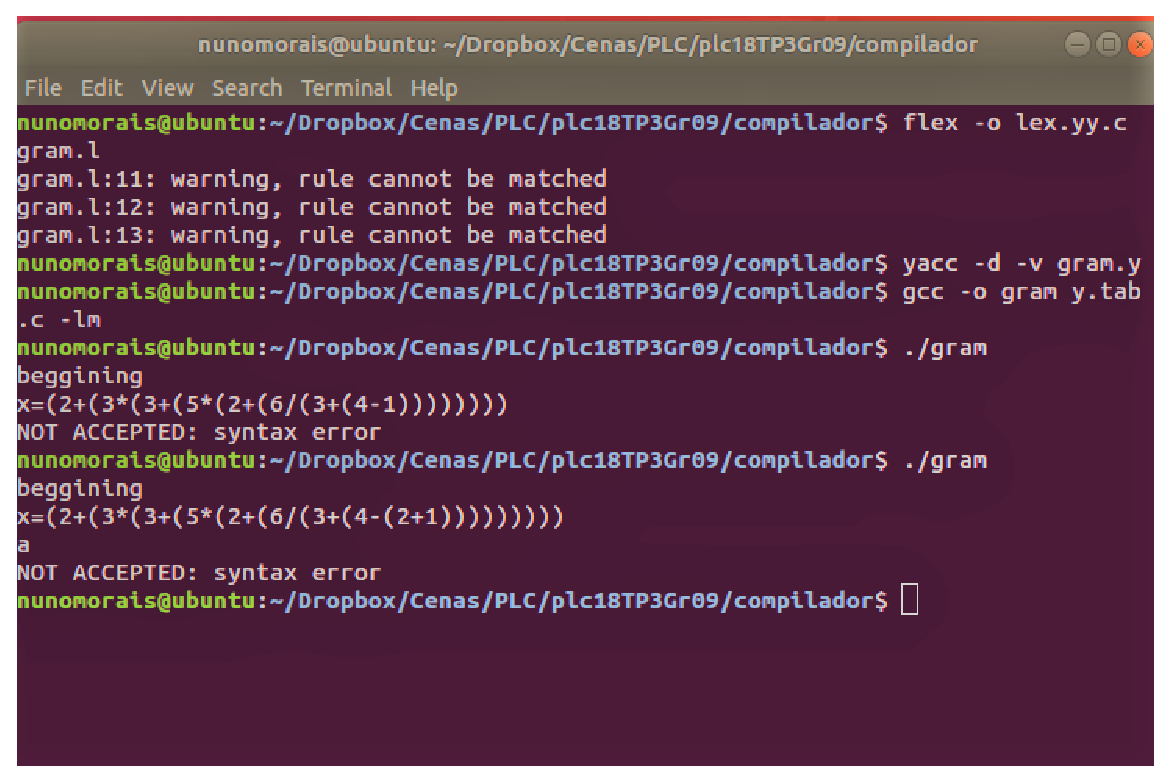
\includegraphics[width=14cm,height= 8cm]{comandos.eps}
	\caption{Comandos}
	\label{Exemplo}
\end{figure}

\begin{figure}[ht]
	\centering
	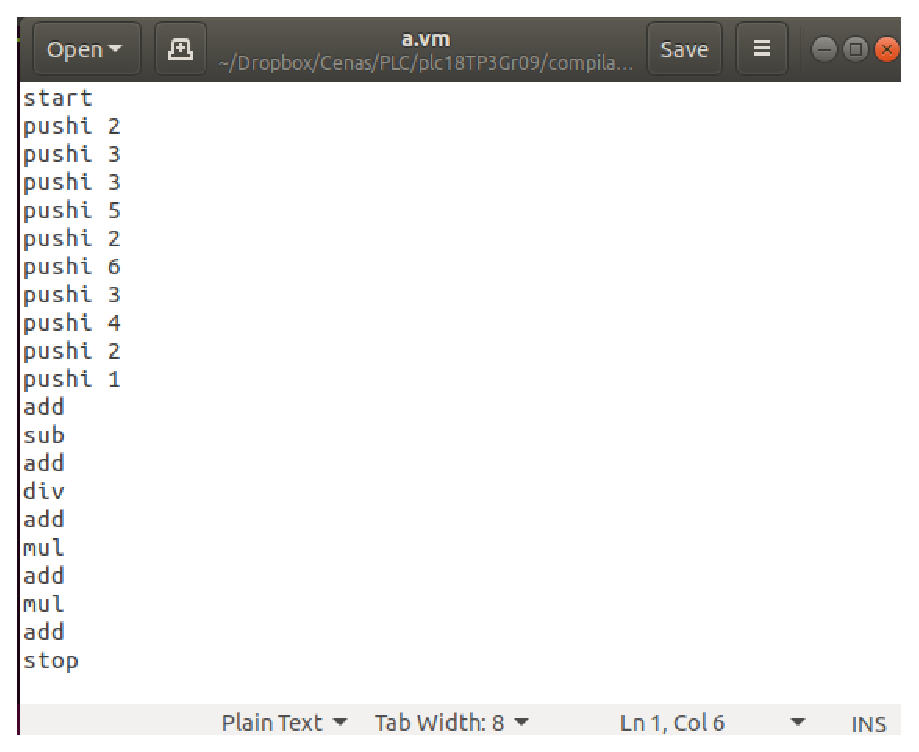
\includegraphics[width=14cm,height= 8cm]{a_vm.eps}
	\caption{a.vm}
	\label{a.vm}
\end{figure}

\begin{figure}[ht]
	\centering
	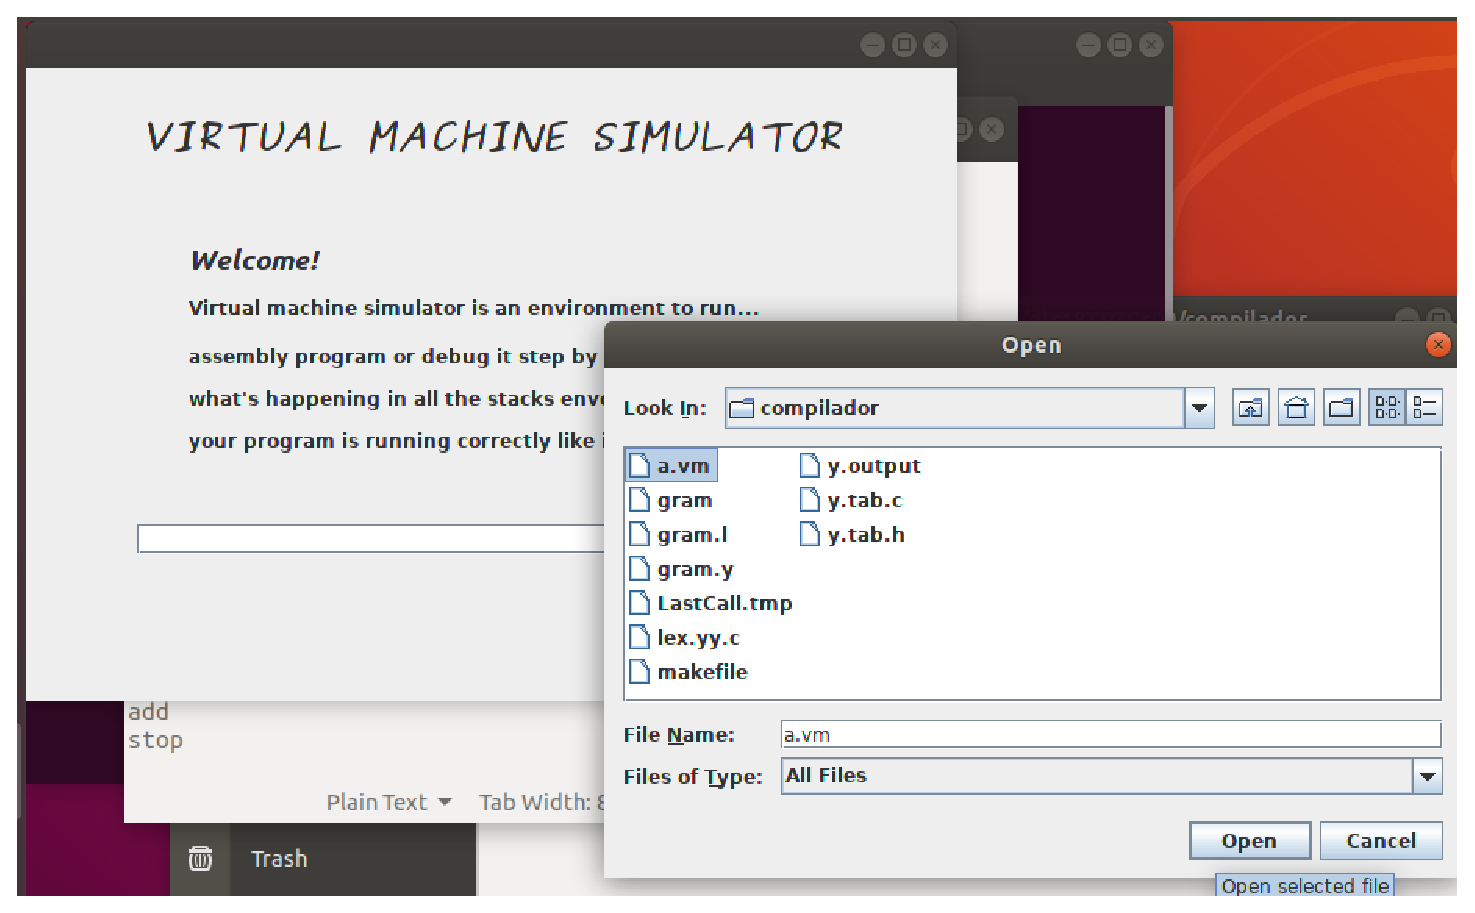
\includegraphics[width=14cm,height= 8cm]{vm1.eps}
	\caption{Maquina Virtual}
	\label{vm1}
\end{figure}

\begin{figure}[ht]
	\centering
	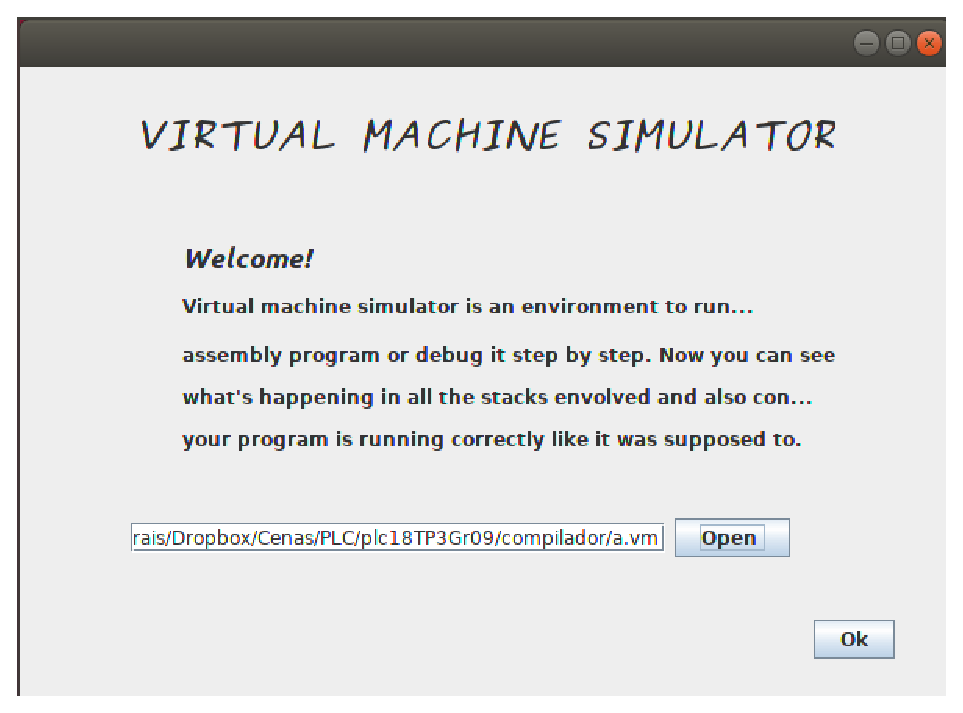
\includegraphics[width=14cm,height= 8cm]{vm2.eps}
	\caption{Maquina Virtual}
	\label{vm2}
\end{figure}

\begin{figure}[ht]
	\centering
	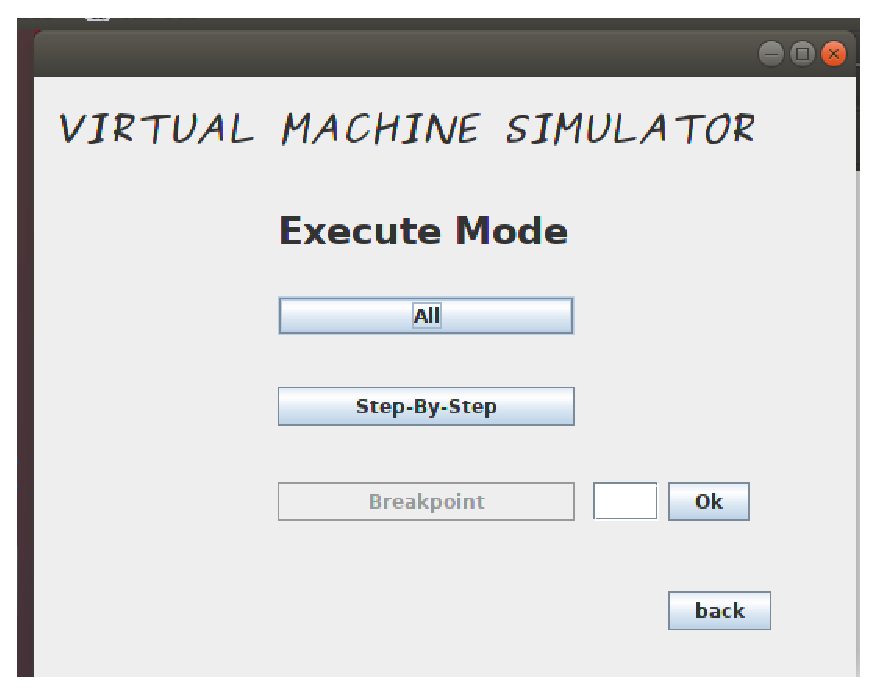
\includegraphics[width=14cm,height= 8cm]{vm3.eps}
	\caption{Maquina Virtual}
	\label{vm3}
\end{figure}

\begin{figure}[ht]
	\centering
	\includegraphics[width=14cm,height= 8cm]{resultado1.eps}
	\caption{Estado Inicial}
	\label{Resutado1}
\end{figure}

\begin{figure}[ht]
	\centering
	\includegraphics[width=14cm,height= 8cm]{resultado2.eps}
	\caption{Estado Final}
	\label{Resultado2}
\end{figure}

\chapter{Codigo do Programa}
Ficheiro gram.l
\begin{code}
%{
#include "y.tab.h"
%}

%%
[=\+\-\*\/%()<>!,;]      { return yytext[0]; }
[a-zA-Z][a-zA-Z0-9]*     { yylval.vals=strdup(yytext); return VAR; }
\"[^"]*\"                { yylval.vals=strdup(yytext); return STR; }
-?[0-9]+                 { yylval.vali=atoi(yytext); return NUMI; }
-?[0-9]+\.[0-9]+         { yylval.valf=atof(yytext); return NUMF; }                
while|WHILE              { return(WHILE); }
if|IF                    { return(IF); }
else|ELSE                { return(ELSE); }
[ ]+AND[ ]+              { return(AND); }
[ ]+OR[ ]+               { return(OR); }
\<=                      { return(LE); }
\>=                      { return(GE); }
==                       { return(EQUALS); }
!=                       { return(NE); }
[ \t\n]                  { ; }
.                        { printf("Error: caracter %c not valid\n", yytext[0]); }
%%

int yywrap() {
   return(1);
}
\end{code}
Ficheiro do Yacc
\begin{code}

%{
#include <stdio.h>
#include <stdlib.h>
#include <string.h>
#define MAX 1024

   int yylex();
   int yyerror();
   int top = 0, topl = 0, i = 0;
   int nif[128] = {0}, apif = 0, nwhile[128] = {0}, apwhile = 0;
   int nf = 0, nelemf = 0, infunc = 0;
   FILE* out;
   char* typeFloat = "float";
   char* typeInt = "int";
   char* typeString = "string";

   typedef struct variable{
      char* type;
      char* desig;
      int posStack;
   } *Variable;

   typedef struct expression{
      char* type;
   } *Expression;

   typedef struct func{
      char* desig;
      char* types[128];
      int nt;
   } *Func;

   Variable v[MAX] = {0}, aux = NULL, vl[MAX] = {0};
   Func funcs[128] = {0}, funcx = NULL;
   int qt = 0, qtl = 0;
   char* types[128] = {0};

   int remVarDes (char* desig, Variable v[], int N){
      if(N==0) return -1;
      int a,b=0;
      for(a=0;a<MAX && b<N; a++){
         if(v[a]!=NULL) b++;
         if(strcmp(v[a]->desig, desig)==0){
            v[a]=NULL;
            return N--;
         }
      }
      return -1;
   }

   int insertVar (Variable var, Variable v[], int N){
      N=remVarDes(var->desig,v,N);
      if(N>=MAX) return -1;

      int c;
      for(c=0;c<MAX;c++){
         if(v[c]==NULL) break;
      }
      v[c]=var;
      return N++;
   }

   int remVar (Variable var, Variable v[], int N){
      if(N==0) return -1;
      int d, e=0;
      for(d=0;d<MAX && e<N;d++){
         if(v[d]!=NULL) e++;
         if(v[d]->posStack == var->posStack){
          v[d] = NULL;
          return N--;
         }
      }
      return -1;
   }

   Variable createVar (char* type, char* desig, int posStack){
      Variable var = (Variable)malloc(sizeof(struct variable));
      var->type = type;
      var->desig = desig;
      var->posStack = posStack;
      return var;
   }

   int isapont (char* t){
	    int i;
	    for (i=0; t[i]!='\0'; i++);
	    return t[i-1]=='*';
    }

    Variable searchDesig(char* desig, Variable v[], int N){
        int i , q = 0;
        for(i=0; q<N && i<MAX; i++){
            if(v[i]!=NULL) q++;
            if(strcmp(v[i]->desig,desig)==0){
                return v[i];
            }
        }
        return NULL;  
    }

   void push(Variable v){
      if(strcmp(v->type,"int")==0){
         fprintf(out,"pushi 0\n");
      }else if (strcmp(v->type,"float")==0){
         fprintf(out,"pushf 0.0\n");
      }else if (strcmp(v->type,"string")==0){
         fprintf(out,"pushs \"\"\n");
      }else {
         printf("ERROR: type doesnt exist");
      }
   }

   void pushtype(char* type){
      if(strcmp(type,"int")==0){
         fprintf(out,"pushi 0\n");  
      }else if (strcmp(type,"string")==0){
         fprintf(out,"pushs \"\"\n");
      }else if (strcmp(type,"float")==0){
         fprintf(out,"pushf 0.0\n");
      }else {
         printf("ERRO: type doesnt exist");   
      }

    }

   void store(Variable v){
      fprintf(out,"storeg %d\n",v->posStack);
   }

   void storel(Variable v){
        fprintf(out,"storel %d\n",v->posStack);
    }

   void insertfunc(Func func, Func funcs[], int nf){
        funcs[nf] = func;
    }
    
    Func createfunc(char* desig, char* types[], int nt){
        Func func = (Func)malloc(sizeof(struct func));
        func->desig = desig;
        int i;
        for(i=0;i<nt;i++){
            func->types[i] = types[i];
        }
        func->nt = nt;
        return func;
    }

    Func updatefunc(Func func, char* types[], int nt){
        int i;
        for (i=func->nt;i<func->nt+nt;i++){
            func->types[i] = types[i-func->nt];
        }
        func->nt += nt;
        return func;
    }

    Func searchfunc(char* desig, Func funcs[], int nf ){
        int i;
        for(i=0;i<nf;i++){
            if(strcmp(funcs[i]->desig,desig)==0){
                return funcs[i];
            }
        }
        return NULL;
    }

   void clear(Variable vl[], int qtl){
        Variable aux = NULL;
        int i = 0;
        while(i<qtl){
            if(vl[i]){
                aux = vl[i];
                vl[i] = NULL;
                free(aux);
                i++;
            }
        }
    }

%}

%union { char *vals; int vali; float valf; }

%token LE GE EQUALS NE OR AND IF ELSE WHILE STR VAR NUMI NUMF TYPE

%type <vals>STR VAR TYPE
%type <vali>NUMI
%type <valf>NUMF

%type<vals> Func Atrib
%type<vali> Cond
%type<vals> Expr Exp


%%

Prog    : Prog If                               { printf("if\n"); }
        | Prog While                            { printf("while\n"); }
        | Prog Atrib ';'                        { printf("initialize var\n"); }
        | Prog VAR '=' Expr ';'                 { printf("update var\n"); store(searchDesig($2,v,qt)); }
        | Prog Func ';'                         { printf("call func\n"); }
        |                                       { printf("beggining\n"); } 
        ;

Func  : VAR Expr                                { if(strcmp($1,"leri")==0){
                                                    fprintf(out,"read\natoi\n");
                                                    $$ = "int";
                                                  }else if(strcmp($1,"lerf")==0){
                                                    fprintf(out,"read\natof\n");
                                                    $$ = "float";
                                                  }else if(strcmp($1,"lers")==0){
                                                    fprintf(out,"read\n");
                                                    $$ = "string";
                                                  }else if(strcmp($1,"escreveri")==0){
                                                    fprintf(out,"writei\n");
                                                    $$ = "int";
                                                  }else if(strcmp($1,"escrevers")==0){
                                                    fprintf(out,"writes\n");
                                                    $$ = "string";
                                                  }else if(strcmp($1,"escreverf")==0){
                                                    fprintf(out,"writef\n");
                                                    $$ = "float";
                                                  }else if(strcmp($1,"atoi")==0){
                                                    fprintf(out,"atoi\n");
                                                    $$ = "int";
                                                  }else if(strcmp($1,"atof")==0){
                                                    fprintf(out,"atof\n");
                                                    $$ = "float";
                                                  }else if(strcmp($1,"ftoi")==0){
                                                    fprintf(out,"ftoi\n");
                                                    $$ = "int";
                                                  }else if(strcmp($1,"itof")==0){
                                                    fprintf(out,"itof\n");
                                                    $$ = "float";
                                                  }else if(strcmp($1,"stri")==0){
                                                    fprintf(out,"stri\n");
                                                    $$ = "string";
                                                  }else if(strcmp($1,"strf")==0){
                                                    fprintf(out,"strf\n");
                                                    $$ = "string";
                                                  }else{
                                                    funcx = searchfunc($1,funcs,nf);
                                                    if(!funcx){
                                                        printf("ERROR: function not found\n");
                                                    }else{
                                                        $$ = funcx->types[0];
                                                        pushtype(funcx->types[0]);
                                                        for(i=0;i<nelemf;i++){
                                                            fprintf(out,"pushl %d\n",top+nelemf-i-1);
                                                        }
                                                        fprintf(out,"pusha %s\ncall\nnop\npop %d\n",$1,nelemf);
                                                        for(i=0;i<nelemf;i++){
                                                           fprintf(out,"swap\npop 1\n");
                                                        }
                                                    }
                                                  }
                                                }
        ;



Atrib   : TYPE VAR                              { if(infunc){
                                                    aux = createVar($1,$2,topl++);
                                                    insertVar(aux, vl, qtl++);
                                                    push(aux); push(aux); storel(aux);
                                                  }
                                                  else{
                                                    aux = createVar($1,$2,top++);
                                                    insertVar(aux, v, qt++); 
                                                    push(aux); push(aux); store(aux);
                                                  } 
                                                } 
        
        | Equal                                 { ; }       
        ;

Equal   : TYPE VAR '='                          { if(infunc){
                                                    aux = createVar($1,$2,topl++);
                                                    insertVar(aux, vl, qtl++);
                                                    push(aux);
                                                  }
                                                  else{
                                                    aux = createVar($1,$2,top++); 
                                                    insertVar(aux, v, qt++);
                                                    push(aux);
                                                  }
                                                }
        | Equal Expr                            { if(infunc){
                                                    storel(aux);
                                                  }
                                                  else{
                                                    store(aux);
                                                  } 
                                                }
        ;


If      : IF Cond               { fprintf(out, "jz endif%d\n",nif[apif]); apif++; nif[apif] = nif[apif-1]+1; }
        | IF '{' Prog '}' ELSE  { apif--; fprintf(out, "jump endif%d\nendif%d:\n",nif[apif+1],nif[apif]);
                                nif[apif] = nif[apif+1]; apif++; nif[apif] = nif[apif-1]+1; 
                                }
        | IF '{' Prog '}'       { apif--; fprintf(out, "endif%d:\n",nif[apif]); nif[apif] = nif[apif+1]; }
        ;

While   : WHILE          { fprintf(out,"while%d:\n",nwhile[apwhile]); }
        | WHILE Cond     { fprintf(out,"jz endwhile%d\n",nwhile[apwhile]); apwhile++; 
                          nwhile[apwhile] = nwhile[apwhile-1]+1; }
        | WHILE '{' Prog '}' { apwhile--; fprintf(out,"jump while%d\nendwhile%d:\n",nwhile[apwhile],
        nwhile[apwhile]); nwhile[apwhile]= nwhile[apwhile+1]; 
                             }
        ;

Cond    : NUMI                      { fprintf(out,"pushi %d\n",$1!=0); }
        | '(' Expr EQUALS Expr ')'  { fprintf(out,"equals\n"); }
        | '(' Expr NE Expr ')'      { fprintf(out,"equals\npushi 0\nequals\n"); }
        | '(' Expr '<' Expr ')'     { if(strcmp($2,"int")==0 && strcmp($4,"int")==0){
                                                    fprintf(out,"inf\n");
                                                  }else if(strcmp($2,"float")==0 && strcmp($4,"float")==0){
                                                    fprintf(out,"finf\nftoi\n");
                                                  }else{
                                                    printf("ERROR: Can't compare different types.\n");
                                                  }
                                                }
        | '(' Expr '>' Expr ')'          { if(strcmp($2,"int")==0 && strcmp($4,"int")==0){
                                                    fprintf(out,"sup\n");
                                         }else if(strcmp($2,"float")==0 && strcmp($4,"float")==0){
                                                    fprintf(out,"fsup\nftoi\n");
                                                  }else{
                                                    printf("ERROR: Can't compare different types.\n");
                                                  }
                                         }
        | '(' Expr LE Expr ')'           { if(strcmp($2,"int")==0 && strcmp($4,"int")==0){
                                                    fprintf(out,"infeq\n");
                                         }else if(strcmp($2,"float")==0 && strcmp($4,"float")==0){
                                                    fprintf(out,"finfeq\nftoi\n");
                                                  }else{
                                                    printf("ERROR: Can't compare different types.\n");
                                                  }
                                         }
        | '(' Expr GE Expr ')'                  { if(strcmp($2,"int")==0 && strcmp($4,"int")==0){
                                                    fprintf(out,"supeq\n");
                                                  }else if(strcmp($2,"float")==0 && strcmp($4,"float")==0){
                                                    fprintf(out,"fsupeq\nftoi\n");
                                                  }else{
                                                    printf("ERROR: Can't compare different types.\n");
                                                  }
                                                }
        | '(' Cond AND Cond ')'                 { fprintf(out,"mul\n"); }
        | '(' Cond OR Cond ')'                  { fprintf(out,"add\n"); }
        | '!' Cond                              { fprintf(out,"pushi 0\nequals\n"); }
        ;

Expr  : '(' Expr '+' Expr ')'               { if(strcmp($2,"int")==0 && strcmp($4,"int")==0){
                                                    fprintf(out,"add\n");
                                                    $$ = $2;
                                                  }else if(strcmp($2,"float")==0 && strcmp($4,"float")==0){
                                                    fprintf(out,"fadd\n");
                                                    $$ = $2;
                                                  }else if(strcmp($2,"string")==0 && strcmp($4,"string")==0){
                                                    fprintf(out,"concat\n");
                                                    $$ = $2;
                                                  }else{
                                                    printf("ERROR: Operation can only be one type\n");
                                                  }
                                            }
      | '(' Expr '-' Expr ')'               { if(strcmp($2,"int")==0 && strcmp($4,"int")==0){
                                                 fprintf(out,"sub\n");
                                                 $$ = $2;
                                               }else if(strcmp($2,"float")==0 && strcmp($4,"float")==0){
                                                 fprintf(out,"fsub\n");
                                                 $$ = $2;
                                               }else{
                                                 printf("ERROR: Operation can only be one type\n");
                                               } 
                                            }
      | '(' Expr '*' Expr ')'               { if(strcmp($2,"int")==0 && strcmp($4,"int")==0){
                                                 fprintf(out,"mul\n");
                                                 $$ = $2;
                                               }else if(strcmp($2,"float")==0 && strcmp($4,"float")==0){
                                                 fprintf(out,"fmul\n");
                                                 $$ = $2;
                                               }else{
                                                 printf("ERROR: Operation can only be one type\n");
                                               } 
                                            }
      | '(' Expr '/' Expr ')'               { if(strcmp($2,"int")==0 && strcmp($4,"int")==0){
                                                 fprintf(out,"div\n");
                                                 $$ = $2;
                                               }else if(strcmp($2,"float")==0 && strcmp($4,"float")==0){
                                                 fprintf(out,"fdiv\n");
                                                 $$ = $2;
                                               }else{
                                                 printf("ERROR: Operation can only be one type\n");
                                               } 
                                            }
      | '(' Expr '%' Expr ')'               { if(strcmp($2,"int")==0 && strcmp($4,"int")==0){
                                                 fprintf(out,"mod\n");
                                                 $$ = $2;
                                               }else{
                                                 printf("ERROR: Operation can only be one type\n");
                                               } 
                                            }
      | '(' Expr ')'                        { $$ = $2; }
      | Exp                                 { $$ = $1; }
      ;                                                

Exp   : NUMI           { fprintf(out,"pushi %d\n", $1); $$=typeInt; }
      | NUMF           { fprintf(out,"pushf %f\n", $1); $$=typeFloat; }
      | STR            { fprintf(out,"pushs %s\n", $1); $$=typeString; }
      | Func           { $$=$1; }
      ;

%%

#include "lex.yy.c"

int yyerror(char *s)
{
  fprintf(stderr, "NOT ACCEPTED: %s \n", s);
}

int main() {
  out = fopen("a.vm", "w");
  if (out==NULL){
     printf("Error when trying to open the file!\n");
     exit(1);
  }
  fprintf(out, "start\n");
  yyparse();
  fprintf(out, "stop\n");
  
  fclose(out);
  return(0);
}
\end{code}

\end{document}